\documentclass[mathserif
%, handout
]{beamer}
 
  \useoutertheme{wuerzburg}
  \useinnertheme[outline]{chamfered}
 \usecolortheme{shark}
 \definecolor{MyBackground}{RGB}{243,246,249}
 \setbeamercolor{background canvas}{bg=MyBackground}

 %\usecolortheme[snowy]{owl}
 %\usecolortheme{owl}
 
 %\usetheme{Warsaw}
 %\usecolortheme{spruce}

\usepackage{tabu}
\usepackage{rotating}
\usepackage[]{algorithm2e}
\usepackage{color, colortbl}
%\usepackage{default}
\usepackage{fontspec}
\usepackage{polyglossia} 
\setmainlanguage{vietnamese}
%\setdefaultlanguage{vietnamese} 
%\setmainfont{Palatino}
 \usepackage{wasysym}
\usepackage{pifont}% http://ctan.org/pkg/pifont

\usepackage{multicol}
\usepackage{sidecap}

\usepackage{hyperref}

\usepackage{pgf}    
\usepackage{tikz}
\usetikzlibrary{arrows,automata,decorations.pathmorphing,backgrounds,positioning,fit}
\usepackage{array}
\usepackage{listings}

\usepackage{enumerate}
%\usepackage{amsmath,mathtools}
%		\usepackage{fink}

\usepackage{amsmath,amsthm, amssymb}
\usepackage{microtype}
\usetikzlibrary{arrows,automata}
\usetikzlibrary{decorations.pathmorphing}


\usetikzlibrary{calc}

 

\usetikzlibrary{trees}
\usepackage{listings}

\setbeamertemplate{footline}[frame number]
\setbeamertemplate{navigation symbols}{}%remove navigation symbols

%\usepackage{listingsutf8}

%\setbeameroption{show notes on second screen=right}


  
%\newtheorem{Lemme}{Bổ đề} 
%\newtheorem*{LI}{Lemme d'itération infinie}

%\newtheorem{Proposition}{Mệnh đề}[section]
%\newtheorem{Theorem}{Định lý}[section]
%\newtheorem{Corollaire}{Hệ quả}[section]
%\newtheorem*{Conjecture}{Giả thuyết}
% \newtheorem*{Probleme}{Bài toán}
% \newtheorem*{Fait}{Fait}
% 
% 
% \theoremstyle{definition} \newtheorem{Definition}{Định nghĩa}
% \theoremstyle{definition} \newtheorem{example}{Ví dụ}
% \theoremstyle{remark} \newtheorem*{Remarque}{Chú ý}


\usetikzlibrary{arrows,automata}



\usetikzlibrary{trees}


% \newcommand{\mnvect}[2]
% {
%   \begin{bmatrix}	#1\\#2
%   \end{bmatrix}
% }

\definecolor{olive}{rgb}{0.3, 0.4, .1}
\definecolor{fore}{RGB}{249,242,215}
\definecolor{back}{RGB}{51,51,51}
\definecolor{title}{RGB}{255,0,90}
\definecolor{dgreen}{rgb}{0.,0.7,0. }
\definecolor{gold}{rgb}{1.,0.84,0.}
\definecolor{JungleGreen}{cmyk}{0.99,0,0.52,0}
\definecolor{BlueGreen}{cmyk}{0.85,0,0.37,0}
\definecolor{RawSienna}{cmyk}{0,0.72,1,0.45}
\definecolor{Magenta}{cmyk}{0,1,0,0} 



%

%\setlength{\topmargin}{0cm} \setlength{\oddsidemargin}{0cm}
%\setlength{\evensidemargin}{0cm} \setlength{\textwidth}{17truecm}
%\setlength{\textheight}{21.0truecm}


%\parindent = 3 pt
%\parskip = 12 pt

%\newtheorem*{LI}{Lemme d'itération infinie}



\newtheorem{prprt}{Propriété}
\newtheorem{prpstn}{Mệnh đề}
\newtheorem{thrm}{Định lý}
\newtheorem{lmm}{Bổ đề}

\newtheorem{crllr}{Hệ quả}
\newtheorem{clm}{Fait}
\newtheorem{nt}{Notation}
 
\newtheorem*{cnjctr}{Conjecture}
\newtheorem{prblm}{Problème}
\newtheorem{qstn}{Question}
\newtheorem{fct}{Fait}
%\newtheorem{xmpl}{Exemple}
\newtheorem{rmrk}{Nhận xét}

\theoremstyle{example}
\newtheorem{xmpl}{Ví dụ}
\newtheorem{xrcs}{Bài tập}
  \newtheorem{dfntn}{Định nghĩa}
  

% \declaretheorem[name=Problème]{prblm}
% \declaretheorem[name=Question, style=remark, numbered=no]{qstn}

% \declaretheorem[name=Théorème, numberwithin=section]{thrm}
% \declaretheorem[name=Lemme, sibling=thrm]{lmm}
% \declaretheorem[ name=Propriété, sibling=thrm]{prprt}
% \declaretheorem[ name=Proposition, sibling=thrm]{prpstn}
% \declaretheorem[name=Corollaire, sibling=thrm]{crllr}
% \declaretheorem[name=Fait, sibling=thrm]{fct}
% \declaretheorem[name=Notation, sibling=thrm]{nt}


% \declaretheorem[style=definition, name=Définition, sibling=thrm]{dfntn}

% %\theoremstyle{definition} \newtheorem{dfntn}{Définition}[section]

% \renewcommand\thmcontinues[1]{reprise de p.\,\pageref{#1}}

% \declaretheorem[style=remark, name=Exemple%, numberwithin=section
% ]{xmpl}

% \declaretheorem[style=remark, name=Remarque, numbered=no]{rmrk}

% %\declaretheorem[style=definition,numberwithin=chapter,name = Exemple]{xmpl}

% %\theoremstyle{remark} \newtheorem{xmpl}{Exemple}[chapter]

% %\theoremstyle{remark} \newtheorem*{rmrk}{Remarque}



\newtheorem{cs}{Cas}


\def\mclose{\texttt{close}}
\def\mopen{\texttt{open}}

\def\mmclose{\texttt{\scriptsize close}}
\def\mmopen{\texttt{\scriptsize open}}



% \newcommand{\mvect}[2]
% {
% \bigl[ \begin{smallmatrix}
% #1\\ #2
% \end{smallmatrix} \bigr]
% }

% \newcommand{\mnvect}[2]
% {
%   \begin{bmatrix}	#1\\#2
%   \end{bmatrix}
% }

% % \newcommand{\mnvect}[2]
% % {
% % #1/#2
% %   % \begin{bmatrix}	#1\\#2
% %   % \end{bmatrix}
% % }

% \newcommand{\XMPL}[3]
% {
%   \begin{xmpl}
%     Soient $L=\{#1\}$ et $\Sigma=\{#2\}$. On peut vérifier que $L$ est \orl\ avec le
%     relateur de base $#3$.
%   \end{xmpl}
% }

% \newcommand{\XMP}[4]
% {
%   \begin{xmpl}[#4]
%     Soient $L=\{#1\}$ et $\Sigma=\{#2\}$. On peut vérifier que $L$ est \orl\ avec le
%     relateur de base $#3$.
%   \end{xmpl}
% }

% \newcommand{\Pui}[2]
% {
%   #1^{\leq #2}
% }


% % \newcommand{\XMPL1}[4]
% % {
% %   \begin{xmpl}
% %     Soient $L=\{#1\}$ et $\Sigma=\{#2\}$. Il est clair que $L$ est \orl\ avec le
% %     relateur de base $#3$. $L^\omega$ est un 
% %   \end{xmpl}
% % }

% \def\vvs{\vspace{11pt}}
% \def\nni{\noindent}


% \newcommand{\cas}[1]
% {
% \vvs\nni
% \textbf{Cas #1 :}
% }



% \newcommand{\souscas}[1]
% {
% \vvs\nni
% \textbf{Sous-cas #1 :}
% }

% \def\pcom{paire de mots incompatibles}
% \def\wpcom{paire de mots $\infty$-incompatible}

% \def\upcom{une paire de mots incompatibles}
% \def\uwpcom{une paire de mots $\infty$-incompatibles}
% \def\comp{\asymp}

% \def\wg{code générateur}

%  \def\gc{code générateur}

% \def\gcx{codes générateurs}
% \def\Gcx{Codes générateurs }
% \def\ugc{un code générateur}
% \def\Ugc{un Code générateur}

% \def\wgc{$\omega$-code générateur}
% \def\wgcx{$\omega$-codes générateurs}
% \def\wGcx{$\omega$-Codes générateurs }
% \def\wugc{un $\omega$-code générateur}
% \def\wUgc{un $\omega$-code générateur}

% \def\orl {langage à un relateur}

% \def\orlx {langages à un relateur}
% \def\Orlx {Langages à un relateur}
% \def\uorl {un langage à un relateur}


% \def\ugc{un code générateur}

% \def\cp{code préfixe}

% \def\iff{si et seulement si} 
% \def\w{\omega}

% \def\CODE{la proposition~\ref{c3prop23}, $L^\omega$ n'a pas de \gc}
% \def\NOCODE{$L^\omega$ n'a pas de \gc}


\def\vs{}
\def\ni{}





%\setlength{\topmargin}{0cm} \setlength{\oddsidemargin}{0cm}
%\setlength{\evensidemargin}{0cm} \setlength{\textwidth}{17truecm}
%\setlength{\textheight}{21.0truecm}


%\parindent = 3 pt
%\parskip = 12 pt

%\newtheorem*{LI}{Lemme d'itération infinie}



\newtheorem{prprt}{Propriété}
\newtheorem{prpstn}{Mệnh đề}
\newtheorem{thrm}{Định lý}
\newtheorem{lmm}{Bổ đề}
\newtheorem{rl}{Luật}

\newtheorem{crllr}{Hệ quả}
\newtheorem{clm}{Khẳng định}
\newtheorem{nt}{Notation}
 
\newtheorem*{cnjctr}{Giả thuyết}

\newtheorem{fct}{Fait}
%\newtheorem{xmpl}{Exemple}

\theoremstyle{example}
\newtheorem{xmpl}{Ví dụ}
\newtheorem{xrcs}{Bài tập}
  \newtheorem{dfntn}{Định nghĩa}
  \newtheorem{qstn}{Câu hỏi}
\newtheorem{prblm}{Bài toán}  
   \newtheorem{sol}{Lời giải}
\newtheorem{rmrk}{Nhận xét}
  
%  \newtheorem{rmrk}{Định nghĩa}
  

% \declaretheorem[name=Problème]{prblm}
% \declaretheorem[name=Question, style=remark, numbered=no]{qstn}

% \declaretheorem[name=Théorème, numberwithin=section]{thrm}
% \declaretheorem[name=Lemme, sibling=thrm]{lmm}
% \declaretheorem[ name=Propriété, sibling=thrm]{prprt}
% \declaretheorem[ name=Proposition, sibling=thrm]{prpstn}
% \declaretheorem[name=Corollaire, sibling=thrm]{crllr}
% \declaretheorem[name=Fait, sibling=thrm]{fct}
% \declaretheorem[name=Notation, sibling=thrm]{nt}


% \declaretheorem[style=definition, name=Définition, sibling=thrm]{dfntn}

% %\theoremstyle{definition} \newtheorem{dfntn}{Définition}[section]

% \renewcommand\thmcontinues[1]{reprise de p.\,\pageref{#1}}

% \declaretheorem[style=remark, name=Exemple%, numberwithin=section
% ]{xmpl}

% \declaretheorem[style=remark, name=Remarque, numbered=no]{rmrk}

% %\declaretheorem[style=definition,numberwithin=chapter,name = Exemple]{xmpl}

% %\theoremstyle{remark} \newtheorem{xmpl}{Exemple}[chapter]

% %\theoremstyle{remark} \newtheorem*{rmrk}{Remarque}



\newtheorem{cs}{Cas}


\def\mclose{\texttt{close}}
\def\mopen{\texttt{open}}

\def\mmclose{\texttt{\scriptsize close}}
\def\mmopen{\texttt{\scriptsize open}}



% \newcommand{\mvect}[2]
% {
% \bigl[ \begin{smallmatrix}
% #1\\ #2
% \end{smallmatrix} \bigr]
% }

% \newcommand{\mnvect}[2]
% {
%   \begin{bmatrix}	#1\\#2
%   \end{bmatrix}
% }

% % \newcommand{\mnvect}[2]
% % {
% % #1/#2
% %   % \begin{bmatrix}	#1\\#2
% %   % \end{bmatrix}
% % }

% \newcommand{\XMPL}[3]
% {
%   \begin{xmpl}
%     Soient $L=\{#1\}$ et $\Sigma=\{#2\}$. On peut vérifier que $L$ est \orl\ avec le
%     relateur de base $#3$.
%   \end{xmpl}
% }

% \newcommand{\XMP}[4]
% {
%   \begin{xmpl}[#4]
%     Soient $L=\{#1\}$ et $\Sigma=\{#2\}$. On peut vérifier que $L$ est \orl\ avec le
%     relateur de base $#3$.
%   \end{xmpl}
% }

% \newcommand{\Pui}[2]
% {
%   #1^{\leq #2}
% }


% % \newcommand{\XMPL1}[4]
% % {
% %   \begin{xmpl}
% %     Soient $L=\{#1\}$ et $\Sigma=\{#2\}$. Il est clair que $L$ est \orl\ avec le
% %     relateur de base $#3$. $L^\omega$ est un 
% %   \end{xmpl}
% % }

% \def\vvs{\vspace{11pt}}
% \def\nni{\noindent}


% \newcommand{\cas}[1]
% {
% \vvs\nni
% \textbf{Cas #1 :}
% }



% \newcommand{\souscas}[1]
% {
% \vvs\nni
% \textbf{Sous-cas #1 :}
% }

% \def\pcom{paire de mots incompatibles}
% \def\wpcom{paire de mots $\infty$-incompatible}

% \def\upcom{une paire de mots incompatibles}
% \def\uwpcom{une paire de mots $\infty$-incompatibles}
% \def\comp{\asymp}

% \def\wg{code générateur}

%  \def\gc{code générateur}

% \def\gcx{codes générateurs}
% \def\Gcx{Codes générateurs }
% \def\ugc{un code générateur}
% \def\Ugc{un Code générateur}

% \def\wgc{$\omega$-code générateur}
% \def\wgcx{$\omega$-codes générateurs}
% \def\wGcx{$\omega$-Codes générateurs }
% \def\wugc{un $\omega$-code générateur}
% \def\wUgc{un $\omega$-code générateur}

% \def\orl {langage à un relateur}

% \def\orlx {langages à un relateur}
% \def\Orlx {Langages à un relateur}
% \def\uorl {un langage à un relateur}


% \def\ugc{un code générateur}

% \def\cp{code préfixe}

% \def\iff{si et seulement si} 
% \def\w{\omega}

% \def\CODE{la proposition~\ref{c3prop23}, $L^\omega$ n'a pas de \gc}
% \def\NOCODE{$L^\omega$ n'a pas de \gc}


\def\vs{}
\def\ni{}


\def\trail{hành trình đơn}
\def\Trail{Hành trình đơn}

\def\ctrail{\trail\ đóng}
\def\Ctrail{\Trail\ đóng }

\def\walk{hành trình}
\def\Walk{Hành trình}

\def\cwalk{hành trình đóng}
\def\Cwalk{Hành trình đóng}

\def\path{đường đi}
\def\Path{Đường đi}
 
\def\conn{liên thông}
\def\Conn{Liên thông}

\def\Comp{Thành phần liên thông}
\def\comp{thành phần liên thông}

\def\Cuted{Cạnh cắt}
\def\cuted{cạnh cắt}

\def\Cutve{Đỉnh cắt}
\def\cutve{đỉnh cắt}

\def\Induced{Đồ thị con cảm sinh}
\def\induced{đồ thị con cảm sinh}

 
\def\iff{{\color{blue} nếu và chỉ nếu}}

\def\ideg{\text{indeg}}
\def\odeg{\text{outdeg}}

\def\pr{\mathrm{Pr}}
\def\ex{\mathrm{Ex}}
\def\S{\mathcal{S}}
\def\var{\mathrm{Var}}

\def\F{\mathbb{F}}
\def\Z{\mathbb{Z}}
\def\N{\mathbb{N}}
\def\ord{\mathrm{ord}}
\newcommand{\bigO}{\ensuremath{\mathcal{O}}}% big-O notation/symbol


 \newcommand{\defi}[1]{{\color{blue}{\textbf{\emph{#1}}}}}
\newcommand{\contradiction}{{\hbox{%
    \setbox0=\hbox{$\mkern-3mu\times\mkern-3mu$}%
    \setbox1=\hbox to0pt{\hss$\times$\hss}%
    \copy0\raisebox{0.5\wd0}{\copy1}\raisebox{-0.5\wd0}{\box1}\box0
}}}

\newcommand{\cmark}{{\color{blue}\Large\ding{51}}}%
\newcommand{\xmark}{{\color{red}\Large\ding{55}}}%

%\newcommand{\defi}[1]{{\color{blue}{\textbf{\emph{#1}}}}}


 \AtBeginSection[]  
 { 
   \begin{frame}[plain]{Nội dung} 
     \tableofcontents[currentsection,currentsubsection] 
   \end{frame} 
 }  



\begin{document}
% \tikzstyle{every picture}+=[remember picture]

% \tikzstyle{na} = [baseline=-.5ex]

\author{Trần Vĩnh Đức}
%\institute[HUST]{Hanoi University of Science and Technology}



% \newcommand{\cmark}{{\color{blue}\Large\ding{51}}}%
% \newcommand{\xmark}{{\color{red}\Large\ding{55}}}%
\title{Sự độc lập của các sự kiện} 
 \author{Toán Chuyên Đề}
\institute[HUST]{HUST}
 
\maketitle

\begin{frame}{Tài liệu tham khảo}  
  \begin{itemize}
  \item Eric Lehman, F Thomson Leighton \& Albert R Meyer,
    \textit{Mathematics for Computer Science}, 2013
    \href{https://www.seas.harvard.edu/courses/cs20/MIT6_042Notes.pdf}{\color{blue}(Miễn
    phí)}
  \item Michael Mitzenmacher và Eli Upfal, \textit{Probability and Computing}, 2005
  \item  Nguyễn Tiến Dũng và Đỗ Đức Thái, \textit{Nhập Môn Hiện Đại Xác Suất \& Thống Kê}.
%  \item Phan .Đ. Diệu, \textit{Logic toán \& cơ sở toán học}. (2003)  
  \end{itemize}
\end{frame} 

\begin{frame}
	\begin{dfntn}
		Sự kiện $A$ là độc lập với sự kiện $B$ nếu
		\[
			\pr[A\mid B] = \pr[A]
		\]
		hoặc nếu $\pr[B] = 0$.
	\end{dfntn}
	Biết $B$ xảy ra không làm thay đổi xác suất  $A$ xảy ra.
\end{frame}

\begin{frame}
	\begin{xmpl}
		Tung hai đồng xu độc lập 
		\begin{align*}
			A &= \text{ sự kiện đồng xu $1$ ngửa}\\
			B &= \text{ sự kiện đồng xu $2$ ngửa}
		\end{align*}
	Ta có
	\[
		\pr[A\mid B] = \pr[A] = 1/2
	\]
	\end{xmpl}
	
\end{frame}
%--- Next Frame ---%

\begin{frame}
	\begin{qstn}
		Hai sự kiện rời nhau có luôn độc lập?
	\end{qstn}
	
\end{frame}
%--- Next Frame ---%

\begin{frame}
	\begin{thrm}
		Sự kiện $A$ là độc lập với sự kiện $B$ nếu và chỉ nếu 
		\[
			\pr[A \cap B] = \pr[A] \cdot \pr[B]
		\]
	\end{thrm}
	\begin{proof}
		\begin{itemize}
			\item Nếu $\pr[B] = 0$, vậy thì 
			\[
				\pr[A\cap B] =  0 = \pr[A]\cdot \pr[B].
			\]
			\item Nếu $\pr[B] > 0$, vậy thì 
			\begin{align*}
				&\pr[A\mid B] = \frac{\pr[A\cap B]}{\pr[B]} = \pr[B] \\
				\Longleftrightarrow\qquad  &\pr[A \cap B] = \pr[A]\cdot \pr[B] 
			\end{align*} 
		\end{itemize}
		
		\vspace{-0.5cm}
	\end{proof}
\end{frame}

\begin{frame}
	\begin{crllr}[Tính đối xứng]
		Sự kiện $A$ độc lập với sự kiện $B$ nếu và chỉ nếu sự kiện $B$ độc lập với sự kiện $B$.
	\end{crllr}
\end{frame}
%--- Next Frame ---%

\begin{frame}
	\begin{qstn}
		Tung hai đồng xu độc lập 
		\begin{align*}
			A &= \text{ sự kiện chúng cùng mặt}\\ 
			B &= \text{ sự kiện đồng xu thứ nhất ngửa}
		\end{align*}
		Hỏi sự kiện $A$ có độc lập với sự kiện $B$? 
	\end{qstn}
\end{frame}
%--- Next Frame ---%

\begin{frame}
	\begin{qstn}
		Xét hai đồng xu với tính chất 
		\[
			\pr[H] = p, \qquad \pr[T] = 1 - p.
		\]
		Xét hai sự kiện
		\begin{align*}
			A &= \text{ sự kiện chúng cùng mặt}\\ 
			B &= \text{ sự kiện đồng xu thứ nhất ngửa}
		\end{align*}
		Với những giá trị nào của $p$ thì hai sự kiện này độc lập?
	\end{qstn}
\end{frame}
%--- Next Frame ---%

\begin{frame}
	\begin{dfntn}
		Các sự kiện $E_1, E_2, \dots, E_n$ là độc lập nếu, với mọi tập con $S \subseteq \{1, \dots, n\}$, 
		\[
			\pr\left[\bigcap_{j\in S} E_j \right] = \prod_{j \in S}\pr[E_j].
		\] 
	\end{dfntn}
	\begin{xmpl}
		Khi $n = 3$: các sự kiên $E_1, E_2, E_3$ là độc lập nếu 
		\begin{align*}
			\pr[E_1 \cap E_2] &= \pr[E_1]\cdot \pr[E_2]\\
			\pr[E_1 \cap E_3] &= \pr[E_1]\cdot \pr[E_3]\\
			\pr[E_2 \cap E_3] &= \pr[E_2]\cdot \pr[E_3]\\
			\pr[E_1 \cap E_2 \cap E_3] &= \pr[E_1]\cdot \pr[E_2] \cdot \pr[E_3]
		\end{align*}
	\end{xmpl}
\end{frame}
%--- Next Frame ---%

\begin{frame}
	\begin{xmpl}
		Tung ba đồng xu độc lập
		\begin{align*}
			A_1 = \text{ sự kiện kết quả đồng 1 giống kết quả đồng 2}\\
			A_2 = \text{ sự kiện kết quả đồng 2 giống kết quả đồng 3}\\
			A_3 = \text{ sự kiện kết quả đồng 3 giống kết quả đồng 1}
		\end{align*} 
		Có phải các sự kiện này độc lập? 
	\end{xmpl}
\end{frame}
%--- Next Frame ---%

\begin{frame}
	\begin{dfntn}
		Các sự kiện $E_1, E_2, \dots, E_n$ là độc lập từng đôi một nếu, với mọi  $i, j \in \{1,2,\dots, n\}$, $i\not=j$, 
		\[
			\pr[E_i \cap E_j] = \pr[E_i]\cdot \pr[E_j].
		\] 
	\end{dfntn}
\end{frame}
%--- Next Frame ---%

\begin{frame}
	\begin{block}{Bài toán ngày sinh nhật}
		Một lớp học bất kỳ có $30$ sinh viên. Xác suất để ít nhất hai người trong lớp trùng ngày sinh nhật  là bao nhiêu?
	\end{block}
\end{frame}
%--- Next Frame ---%

\begin{frame}{Không ai trùng ngày sinh}
	\begin{itemize}
		\item Nếu đã có một người trong phòng, người thứ $2$ vào phòng, xác suất chị ta có ngày sinh khác với người đầu tiên là $(1 - 1/365)$.
		\item Người thứ $3$ vào phòng, xác suất anh ta có  khác với hai người trong phòng là $(1 - 2/365)$ 
		\item Giả sử trong phòng đã có $k-1$ người khác ngày sinh nhật. Khi người thứ $k$ vào phòng, xác suất chị ta có ngày sinh khác với $k-1$ người trong phòng là $(1 - (k-1)/365)$.  
		\item  Vậy xác suất $30$ người trong phòng có ngày sinh nhật đôi một khác nhau là 
		\[
			\left(1 - \frac{1}{365}\right) \cdot \left(1 - \frac{2}{365}\right) \cdot \left(1 - \frac{3}{365}\right) \cdots \left(1 - \frac{29}{365}\right) \approx 0.2937
		\] 
	\end{itemize}
\end{frame}
%--- Next Frame ---%

\begin{frame}
	Khai triển Taylor của hàm $e^{-x}$ là 
	\[
		e^{-x} = 1 - x + \frac{x^2}{2!} - \cdots.
	\]
	Vậy khi $x<1$, ta có 
	\[
		1 - x \leq e^{-x}.
	\]
\end{frame}
%--- Next Frame ---%
\begin{frame}{Tổng quát hoá}
Nếu có $m$ người và $n$ ngày sinh có thể, vậy xác suất để mọi người có ngày sinh khác nhau là 
\[
	\left(1 - \frac{1}{n}\right) \cdot \left(1 - \frac{2}{n}\right) \cdot \left(1 - \frac{3}{n}\right) \cdots \left(1 - \frac{m-1}{n}\right) = \prod_{j=1}^{m-1} \left(1 - \frac{j}{n}\right)
\]
Dùng công thức $1-k/n \approx e^{-k/n}$ khi $k$ nhỏ so với $n$, ta được 
\begin{align*}
		\prod_{j=1}^{m-1} \left(1 - \frac{j}{n}\right) &\approx \prod_{j=1}^{m-1} e^{-j/n}\\
			                                           &= \exp\left(-\sum_{j=1}^{m-1} \frac{j}{n}\right)\\
													   &=\exp\left(-m(m-1)/2n\right)\\
													   &\approx \exp(-m^2/2n) 
\end{align*}
	
\end{frame}
%--- Next Frame ---%
\begin{frame}{Khi xác suất trùng ngày sinh gần $1/2$}
	\begin{itemize}
		\item 	Giá trị của $m$ từ phương trình 
	\[
		\frac{m^2}{2n} = \ln 2\quad \Longleftrightarrow\quad m = \sqrt{2n\ln 2} \approx 1.1774 \sqrt{n}. 
	\]
	đảm bảo rằng "xác suất $m$ người có ngày sinh nhật khác nhau là $1/2$".
	
	
	
	\item Trong trường hợp $n=365$, ta được $m = 22.49$.  Có nghĩa rằng:
	\begin{block}{}
	 Trong một nhóm gồm $23$ người, xác suất để có hai người trùng ngày sinh ít nhất bằng $1/2$.		
	\end{block}

	\end{itemize}

\end{frame}
%--- Next Frame ---%

\begin{frame}
	\begin{block}{Nguyên lý ngày sinh nhật}
		Nếu một năm có $d$ ngày và có $\sqrt{2d}$ người trong phòng, vậy thì xác suất có hai người cùng ngày sinh nhật khoảng $1 - 1/e \approx 0.632$.
	\end{block}

\end{frame}
% %--- Next Frame ---%

\begin{frame}{Đánh giá thô}
\begin{itemize}
	\item Đặt $E_k = $ sự kiện ngày sinh người thứ $k$ {\color{red}không} trùng với $k-1$ người trước đó. 

	\item Xác suất $k$ người đầu tiên có trùng ngày sinh là
	\begin{align*}
		\pr [\overline{E_1} \cup \overline{E_1} \cup \cdots \cup \overline{E_k} ] &\leq \sum_{i=1}^{k} \pr[E_i]\\
		                                                                          &\leq \sum_{i=1}^{k} \frac{i-1}{n}\\
																				  &=  \frac{k(k-1)}{2n}\\
	\end{align*}
	
	\vspace{-0.3cm}
	\begin{block}{}
		Với $\left\lfloor \sqrt{n}\right\rfloor$ người, xác suất ít nhất $1/2$ là mọi ngày sinh nhật của họ đều khác nhau. 
	\end{block}   
	
\end{itemize}
\end{frame}
%--- Next Frame ---%

\begin{frame}{Đánh giá thô (tiếp)}
	\begin{itemize}
		\item Giả sử $\left\lceil\sqrt{n}\right \rceil$ người đầu tiên có ngày sinh nhật khác nhau.
		\item Mỗi người tiếp theo có xác suất $\sqrt{n}/n$ trùng ngày sinh nhật với $\left\lceil \sqrt{n}\right\rceil$ người đầu tiên.
		\item Vậy xác suất $\left\lceil \sqrt{n}\right\rceil$ người tiếp theo có ngày sinh nhất khác với   $\left\lceil\sqrt{n}\right\rceil$ người đầu tiên là 
		\[
			\left(1- \frac{1}{\left\lceil \sqrt{n}\right\rceil}\right)^{\left\lceil \sqrt{n}\right\rceil}<\frac{1}{e} < \frac{1}{2}.
		\]
		\end{itemize}
	\begin{block}{}
		Khi có $2\left\lceil \sqrt{n} \right\rceil$ người, xác suất nhiều nhất  $1/e$ là mọi ngày sinh của họ  đều khác nhau.

	\end{block}
\end{frame}
%--- Next Frame ---%
\begin{frame}{Hàm băm mật mã}
	\begin{dfntn}
	  \textit{Hàm băm}  là hàm tính được một cách ``hiệu quả''
	  \[
	  H: \{\mathtt{0},\mathtt{1}\}^* \rightarrow \{\mathtt{0},\mathtt{1}\}^d.
	  \]
	  Nó ánh xạ   một xâu nhị phân  độ dài bất kỳ trong không gian thông điệp thành một xâu nhị phân độ
	  dài cố định, gọi là \textit{mã băm}.
	\end{dfntn}

	Thông thường độ dài của mã  băm là   $d= 128, 160, 256$ hoặc  $512$ bit.
\end{frame}
%--- Next Frame ---%

\begin{frame}
	\begin{xmpl}
	Một số hàm băm trong thực tế.
	\begin{center}
	  \begin{tabular}[h]{|l|l|}
	\hline 
	    \textbf{Hàm băm} & $d$  \\
	    \hline 
	    MD4, MD5 & $128$ \\
	    SHA-1 & $160$ \\
	    SHA-256 &$256$ \\
	    SHA-512 &$512$\\
	    SHA-3 (Keccak) &$224, 256, 384, 512$ \\
	\hline 
	  \end{tabular}
	\end{center}
	\end{xmpl}
\end{frame}
%--- Next Frame ---%

\begin{frame}{Hàm băm và tính nén}
	\begin{itemize}
		\item 	Giả sử  hàm băm được thiết kế một cách lý tưởng (như ngẫu nhiên), khi đó  cho trước mã băm~$x$, xác suất tìm được   một dữ liệu  $m$ thỏa mãn  $H(m) = x$ chỉ là $2^{-d}$. 
	
	\item Con số này rất gần~$0$ khi $d$ đủ lớn. Như vậy hàm băm cho ta một biểu diễn \textit{nén} hợp lý của dữ liệu.

	\end{itemize}
	
\end{frame}
%--- Next Frame ---%

\begin{frame}
	\begin{block}{}
		\begin{figure}[h]
		  \centering
		    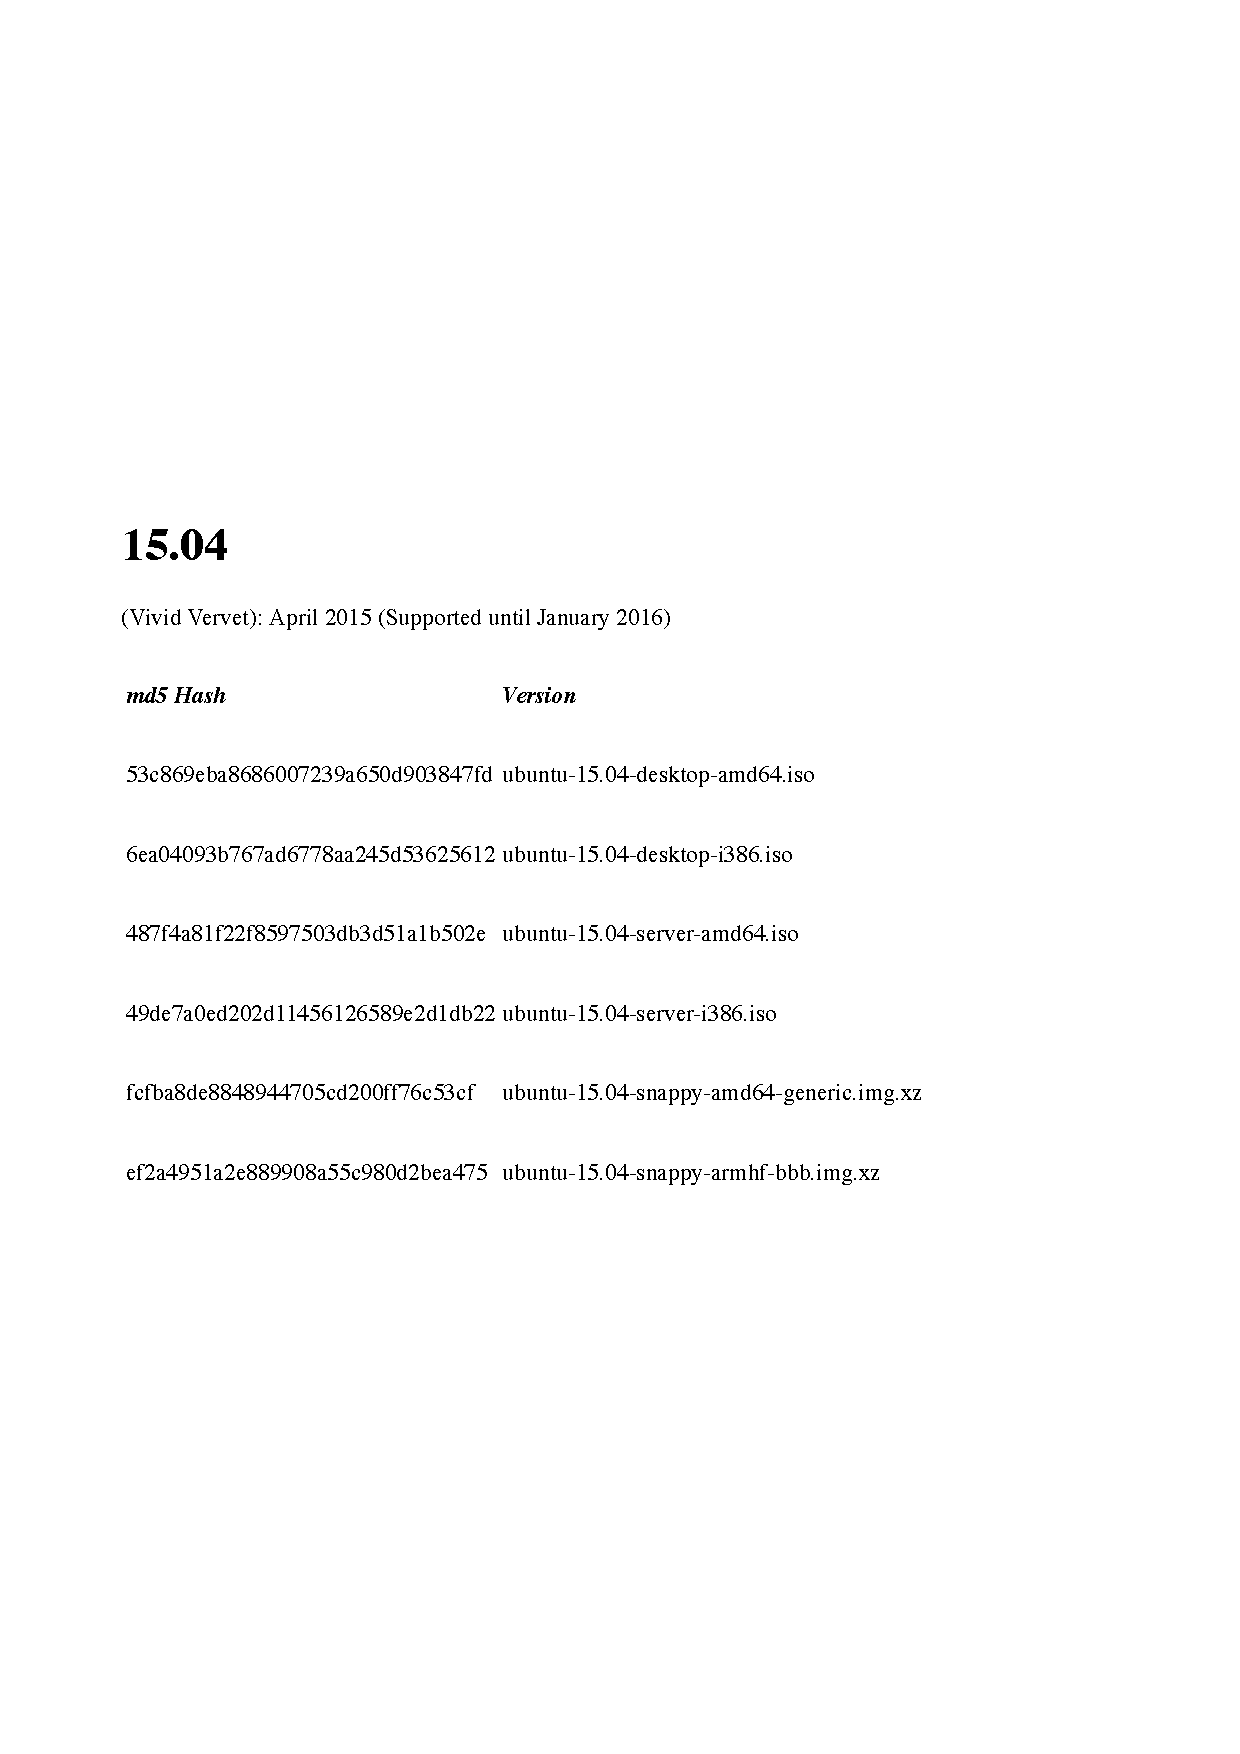
\includegraphics[width=.8\textwidth]{hashUbuntu.pdf}
		\end{figure}
		
	\end{block}
	
\end{frame}
%--- Next Frame ---%

\begin{frame}
	\begin{dfntn}
	  Một \textit{xung đột} cho hàm  $H$ là một cặp $m_0, m_1 \in
	  \{0,1\}^*$ thỏa mãn
	  \[
	  H(m_0) = H(m_1) \quad \text{và}\quad m_0 \not = m_1.
	  \]
	\end{dfntn}
	\begin{itemize}
		\item 	Vì kích thước đầu vào của hàm băm lớn hơn so với kích thước đầu ra, nên theo nguyên lý ``chuồng bồ câu'', luôn tồn tại xung đột. 
		\item Tuy vậy, để hàm băm là an toàn  thì việc tìm thấy xung đột phải  rất ``khó''. Có nghĩa rằng, xác suất tìm thấy xung đột phải ``nhỏ''. 
	\end{itemize}
\end{frame}
%--- Next Frame ---%

\begin{frame}
	\begin{block}{Nguyên lý ngày sinh nhật}
		Xét tập thông điệp $M$ với $|M|> \sqrt{2\cdot 2^d}$ và nếu các giá trị trên $M$ được chọn ngẫu nhiên (đều) và độc lập. Vậy thì
		\[
			\exists x, y \in M\quad  \text{thoả mãn }\quad H(x) = H(y)
		\]
		với xác suất $> 1/2$.
	\end{block}
\end{frame}
%--- Next Frame ---%

\end{document}



%%% Local Variables:
%%% mode: latex
%%% TeX-engine: xelatex	
%%% TeX-master: t
%%% End:
